%% ----------------------------------------------------------------------
\chapter{A false positive: the two candidates of TIC 229701403}
\label{ch:tic2297}

The opposite of a control target is a candidate that turns out not to be a
planet. TIC~229701403 ($T_\mathrm{mag} = 10.97$, a G star of
1.16~$R_\odot$, 258~pc) was found by Roger Dymock in TESS data with two long
period candidates of Saturn size:

\begin{center}
\begin{tabular}{@{}lccccc@{}}
\toprule
 & P (d) & T0 (BTJD) & depth (ppm) & T14 (h) & profile\\
\midrule
b & 490.259 & 1951.170 & 7341 & 10.5 & \code{profile_TIC229701403_b}\\
c & 829.124 & 1857.428 & 5470 & 10.2 & \code{profile_TIC229701403_c}\\
\bottomrule
\end{tabular}
\end{center}

Each profile gives the ephemeris of its own candidate and masks the
transits of the other one (\code{--mask-ephemeris}). The star lies near the
northern ecliptic pole and was observed in 40 sectors between 2019 and 2024;
two of them (59 and 86) are excluded automatically for scattered light.
This chapter shows how the pipeline and the audit flag the candidates, and
how a look at \emph{all} the dips together turns two planets into one
eclipsing binary.

\section*{What the runs say}

Both runs end with \emph{NOT passed}, and the audits list four FAIL each:

\begin{itemize}
\item \textbf{Depth consistency.} The three transits of b have on-target
depths of 8090, 12\,480 and 7290~ppm ($\chi^2_\nu = 281$); those of c 4990
and 4440~ppm, and the third predicted transit of c, in sector 81, is
\emph{absent} ($-460 \pm 150$~ppm).
\item \textbf{Odd/even.} 10$\sigma$ (b) and 15$\sigma$ (c).
\item \textbf{Secondary eclipse.} For b the search finds a second dip at
phase 0.308, 1490~ppm deep: far from 0.5, and deep and warm
(3900~K) --- not the occultation of a planet.
\item \textbf{Centroids.} In every sector with a transit the centroid of the
difference image lies 65$''$ (3 pixels) from the target, at
30$\sigma$, on the neighbour TIC~229701402 ($T_\mathrm{mag} = 11.46$,
5300~K; Figure~\ref{fig:t2297-di}).
\end{itemize}

TRICERATOPS gives FPP~$\approx 1$ for b (mostly SEBx2P) and FPP~0.09 for c.
Neither number is the point: the tests above already say that the
candidates are not what they seem.

\begin{figure}[ht]
\centering
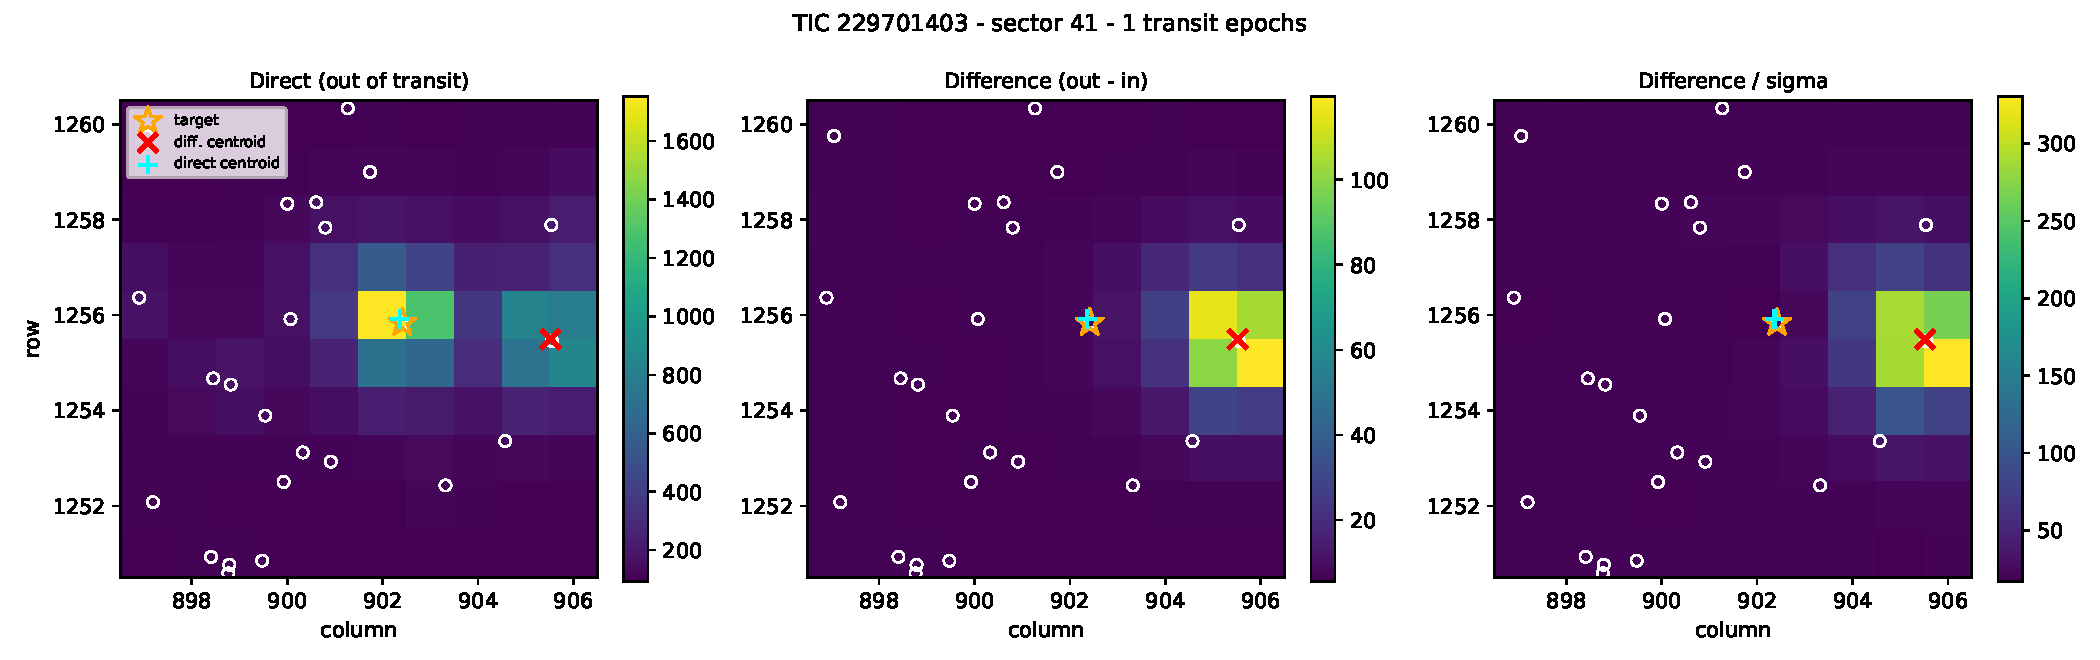
\includegraphics[width=\textwidth]{tic229701403_diffimg_s41.pdf}\\[0.5em]
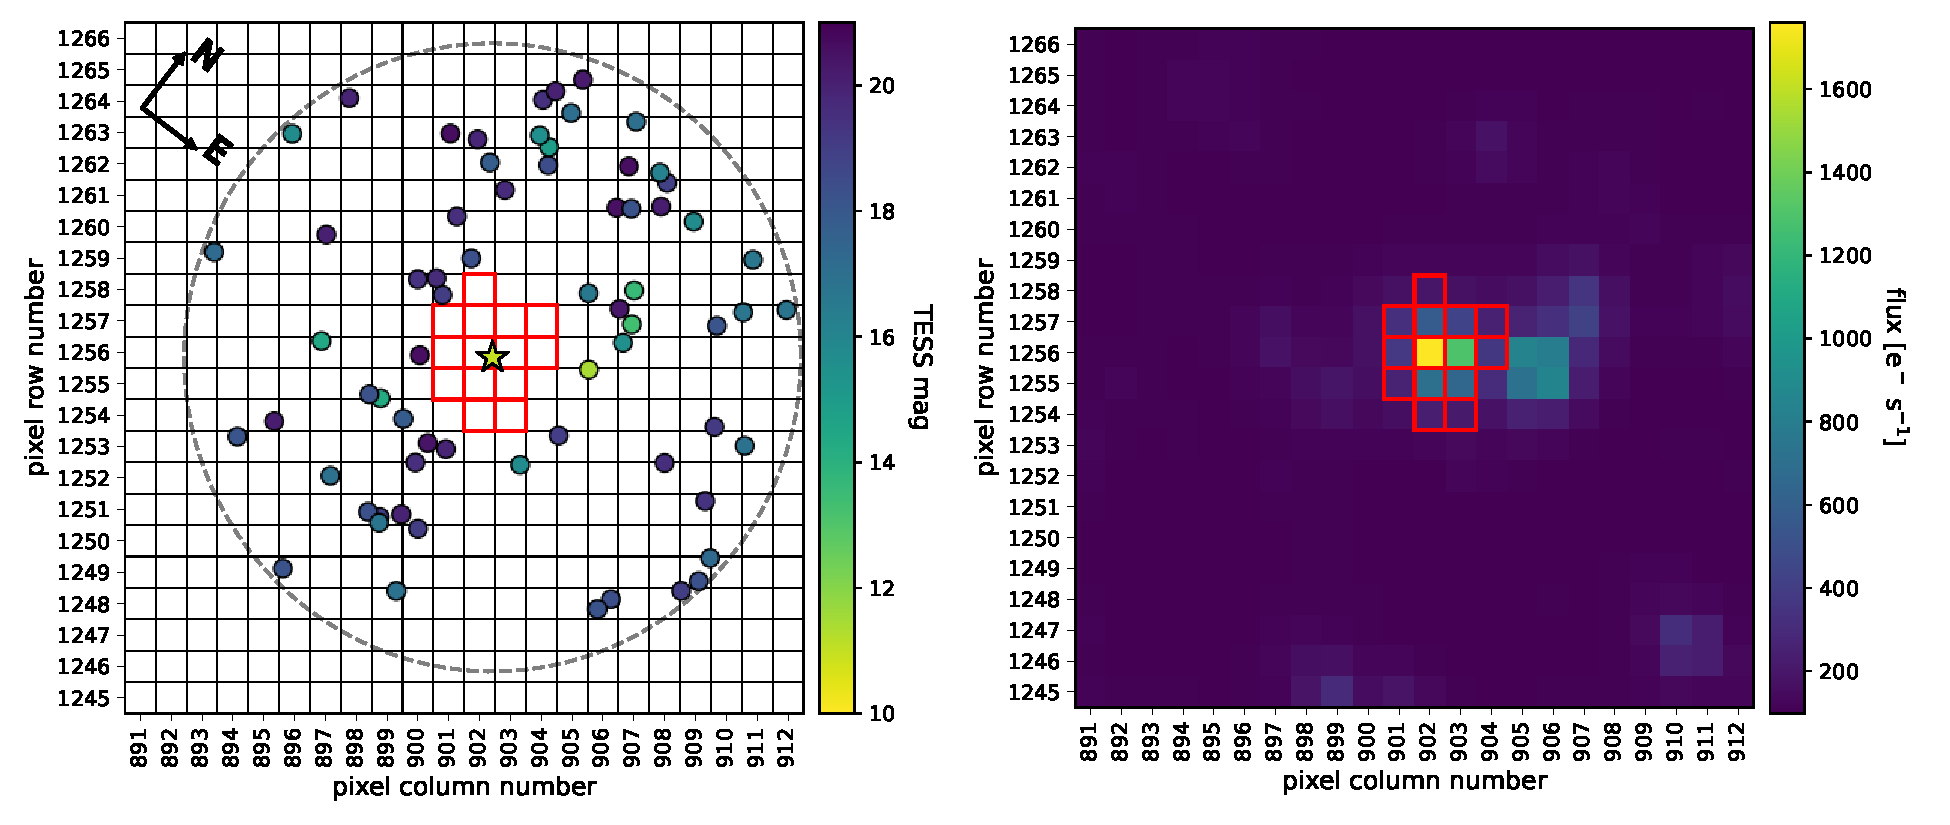
\includegraphics[width=0.75\textwidth]{tic229701403_field_s41.pdf}
\caption{Sector 41, the deepest event (BTJD 2441.43). Top: direct image,
difference image (out of transit minus in transit) and difference over its
error. The target (star symbol) is bright in the direct image, but the
light that disappears comes from the star three pixels to the right, TIC
229701402 (red cross: centroid of the difference image). Bottom: the field
with the optimal aperture (red); the neighbour lies at its edge.}
\label{fig:t2297-di}
\end{figure}

\section*{One period for all dips}

A list of all dips deeper than about 1000~ppm in the 38 good sectors shows
ten clear events. Their times fit a single period of
\textbf{245.13~days}, with the events at two fixed phases
(Figures~\ref{fig:t2297-ecl} and \ref{fig:t2297-time}):

\begin{center}
\begin{tabular}{@{}lll@{}}
\toprule
 & Times (BTJD) & In the aperture\\
\midrule
Primary eclipse, phase 0 & 1706.05, 1951.16, 2441.43, 2686.56, 3421.94 & 3300--9700 ppm\\
Secondary eclipse, phase 0.617 & 1857.39, 2592.76, 2837.93, 3328.20, 3573.29 & 2100--4100 ppm\\
\bottomrule
\end{tabular}
\end{center}

\begin{itemize}
\item The linear fits give $P = 245.1283$~d (primaries, rms 9~min) and
$245.1317$~d (secondaries): the same period.
\item Every predicted eclipse that falls in TESS data is observed; none is
missing. At half the period (122.6~d) no dips are seen, so 245.13~d is the
true period.
\item Candidate \textbf{b} (490.26~d $= 2\times245.13$) used only every
other primary eclipse; the primary at 2686.56 lay between them.
\item Candidate \textbf{c} (829.12~d) joined a secondary eclipse (1857.39)
to a primary (2686.56). Its third ``transit'' was therefore predicted at a
time when nothing happens: the absent event in sector 81.
\item The ``secondary eclipse at phase 0.308'' of the b run is the real
secondary eclipse, seen on the double period:
$0.617/2 = 0.308$.
\item A secondary eclipse at phase 0.617 instead of 0.5 means an eccentric
orbit: $e\cos\omega \approx \tfrac{\pi}{2}(0.617-0.5) = 0.18$.
\end{itemize}

\begin{figure}[ht]
\centering
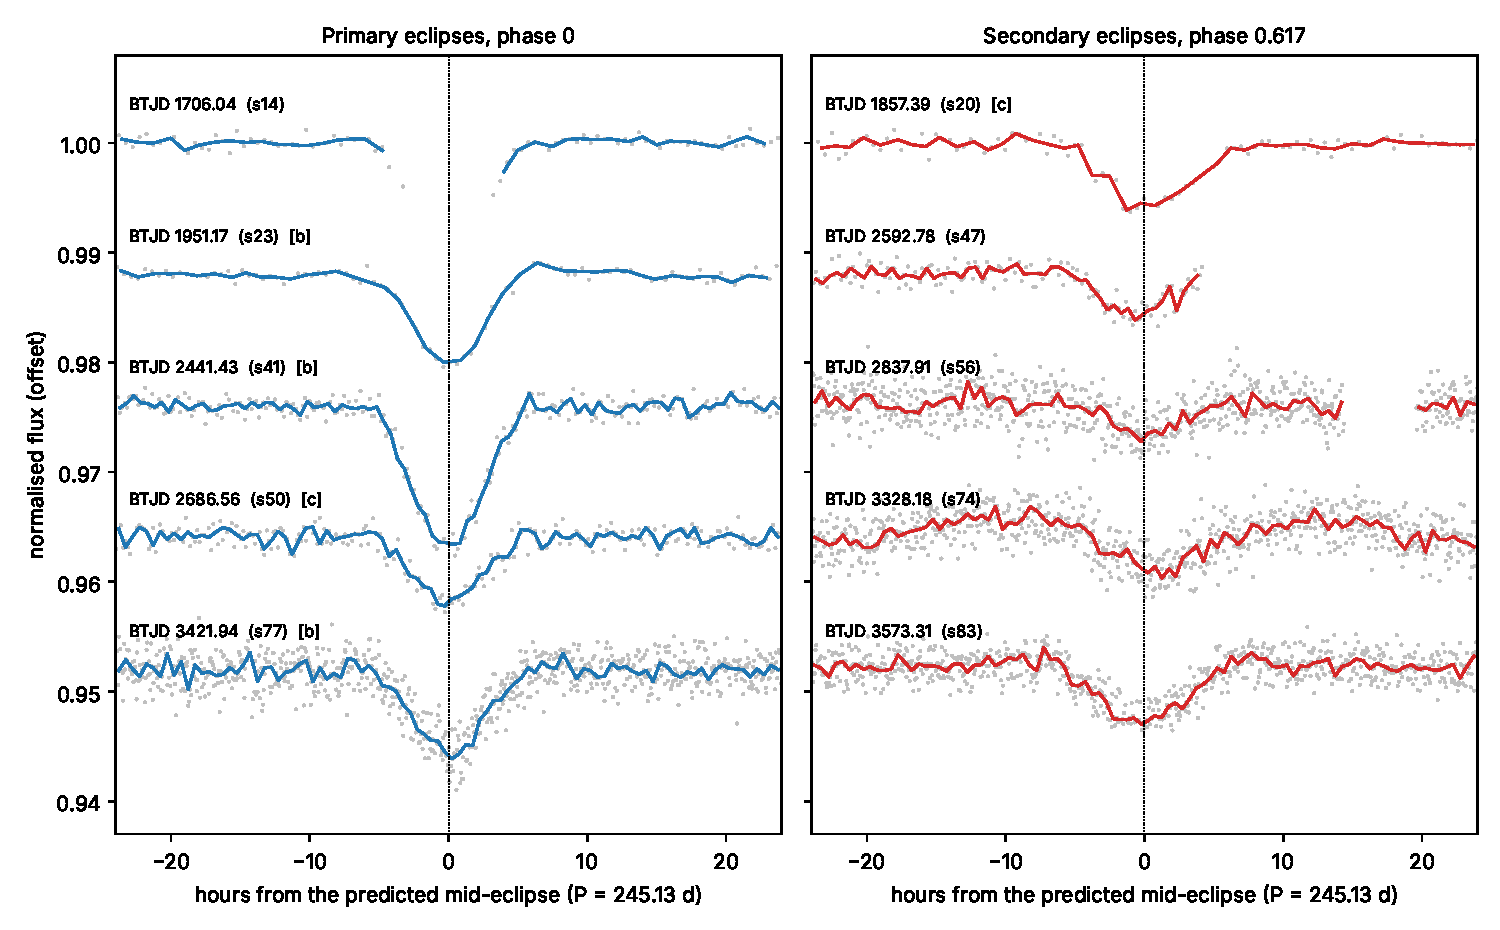
\includegraphics[width=\textwidth]{tic229701403_eclipses.pdf}
\caption{All ten eclipses, centred on the times predicted with
$P = 245.13$~d (pipeline light curves; lines: 30-min to 1-h bins). Left:
primary eclipses, right: secondary eclipses. The labels [b] and [c] mark the
events used by the two candidates. Sector 14 (top left) has a data gap
during the eclipse.}
\label{fig:t2297-ecl}
\end{figure}

\begin{figure}[ht]
\centering
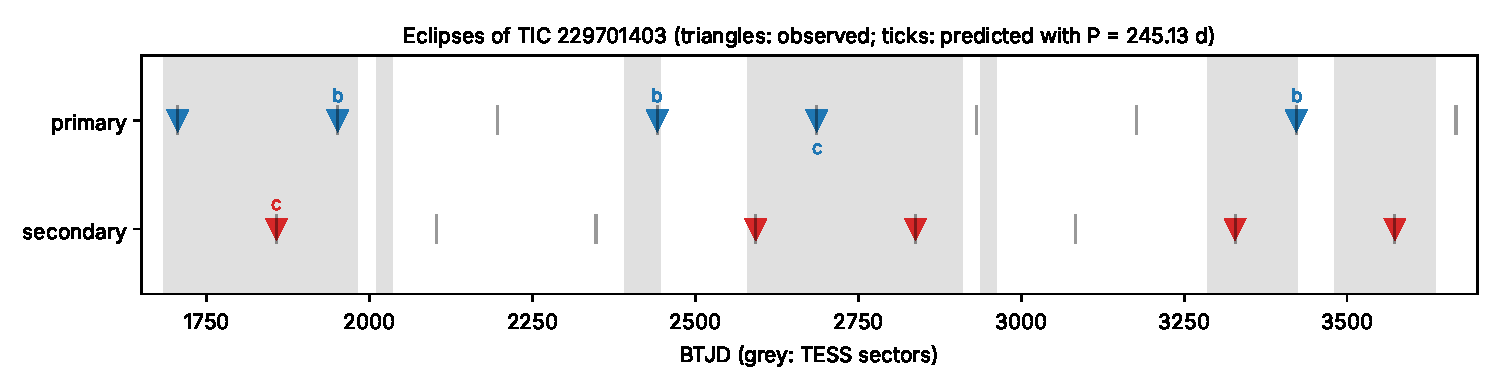
\includegraphics[width=\textwidth]{tic229701403_timeline.pdf}
\caption{Timeline: TESS sectors (grey), observed eclipses (triangles) and
the eclipses predicted with $P = 245.13$~d (ticks). Predicted eclipses
without a triangle fall in gaps between sectors.}
\label{fig:t2297-time}
\end{figure}

\section*{Where the eclipses happen}

The difference images put the source on TIC~229701402, 65$''$ from the
target. That star supplies only 2--4~\% of the light in the TESS aperture,
so to produce dips of 0.3--1~\% it must dim by 20--45~\%: these are
stellar eclipses, not transits. Two observations agree with this:

\begin{itemize}
\item \textbf{The depth changes from sector to sector.} The fraction of the
neighbour's light that falls in the aperture changes with the aperture and
the position of the star on the detector. A dip on the neighbour therefore
has a different depth in every sector; a dip on the target would not.
\item \textbf{The shape is V-like} (audit fold, b run): a grazing or partial
eclipse of two stars, not the flat-bottomed transit of a planet.
\end{itemize}

TRICERATOPS itself gives the neighbour scenarios (NEB, NEBx2P) a low
probability. It models one transit with one depth for all events, which a
signal of varying depth on a star at the edge of the aperture does not
fit. The difference imaging does not need that assumption, which is why
the audit treats its 30$\sigma$ offset as a FAIL.

\section*{What observers can do}

The decisive observation is a ground light curve with \emph{separate
apertures} on TIC~229701403 and TIC~229701402 during an eclipse: at 65$''$
the two stars are easily separated. The neighbour should show an eclipse of
tens of per cent, the target nothing. The star is circumpolar from Europe
(declination $+71.6^\circ$) and bright enough for small telescopes. The
next eclipses (allow $\pm1$~h around mid-eclipse; they last about 10~h):

\begin{center}
\begin{tabular}{@{}lll@{}}
\toprule
Eclipse & Mid-eclipse (BJD\_TDB) & Date (UTC, approx.)\\
\midrule
Primary & 2461402.45 & 27 December 2026, 23~h\\
Secondary & 2461553.80 & 28 May 2027, 07~h\\
Primary & 2461647.58 & 30 August 2027, 02~h\\
\bottomrule
\end{tabular}
\end{center}

Because the eclipse lasts longer than a night, partial coverage with a
good baseline on one side is enough to see a dip of this size. Light curves
in two bands (Section~\ref{sec:multiband}) add the colours of the two
eclipsed stars: the ratio of the primary and secondary depths in each band
gives their temperature ratio.

\begin{tip}
\textbf{Lessons.}
(1)~Several long-period candidates on one star: check whether all their
dips share a common period, with primaries and secondaries.
(2)~A predicted transit that is absent in data that cover it is a strong
sign that the period is wrong.
(3)~Large odd/even differences together with a secondary eclipse far from
phase 0.5 point to an eccentric eclipsing binary at twice (or a fraction
of) the assumed period.
(4)~A difference-image centroid that sits on another star in every sector
outweighs a low TRICERATOPS probability for that star.
(5)~The audit's own fold of these runs was at first a flat line: it read
two sectors that the pipeline had excluded for scattered light. Since
v4.3 the audit leaves out the same sectors as the pipeline and masks the
transits of masked candidates.
\end{tip}
